\documentclass[a4paper,10pt,twoside]{article}
\usepackage[polish]{babel}
\usepackage[utf8]{inputenc}
\usepackage[T1]{fontenc}
\usepackage{indentfirst}
\usepackage[top=2.5cm, bottom=2.5cm, left=2.5cm, right=2.5cm]{geometry}
\usepackage{graphicx}
\usepackage{amsmath}
\usepackage{booktabs}

\begin{document}

\newcommand{\unit}[1]{\thinspace \mathrm{#1}}

\begin{center}
\bgroup
\def\arraystretch{1.5}
\begin{tabular}{|c|c|c|c|c|c|}
	\hline
	EAIiIB & \multicolumn{2}{|c|}{Piotr Morawiecki, Tymoteusz Paszun} & Rok II & {Grupa 3a} & {Zespół 6} \\
	\hline
	\multicolumn{3}{|c|}{\begin{tabular}{c}Temat: Mostek Wheatstone'a \end{tabular}} &
	\multicolumn{3}{|c|}{\begin{tabular}{c}Numer ćwiczenia: 35 \end{tabular}} \\
	\hline
	\begin{tabular}{@{}c@{}}Data wykonania:\\22.11.2017r.\end{tabular} & \begin{tabular}{@{}c@{}}Data oddania:\\29.11.2017r.\end{tabular} &
	\begin{tabular}{c}Zwrot do poprawki:\\\phantom{data} \end{tabular} & \begin{tabular}{c}Data oddania:\\\phantom{data}\end{tabular} &
	\begin{tabular}{@{}c@{}}Data zaliczenia:\\\phantom{data}\end{tabular} & \begin{tabular}{c}Ocena:\\\phantom{ocena}\end{tabular} \\[4ex]
	\hline
\end{tabular}
\egroup
\end{center}


\section{Cel ćwiczenia}

Celem ćwiczenia jest pomiar nieznanych oporów oraz kombinacji ich połączeń.

\section{Wstęp teoretyczny}

Wyznaczenie wartości napięć i prądów w poszczególnych częściach obwodu opiera się na trzech prawach:

\begin{itemize}
  \item I prawo Kirchoffa (prądowe prawo Kirchoffa) - w węzłach sieci, czyli w punktach połączeń trzech lub więcej przewodów, algebraiczna suma prądów wpływających równa jest zeru. 
  \item II prawo Kirchoffa (napięciowe prawo Kirchoffa) - suma różnic potencjałów w zamkniętej pętli obwodu (tzw. oczku) równa się zeru.
  \item Prawo Ohma - stosunek napięcia na końcach przewodu do wartości natężenia prądu jest wartością stałą, nazywaną opornością.
\end{itemize}

Aby znaleźć poszukiwane prądy powyższe warunki zapisujemy w formie układu odpowiedniej liczby niezależnych równań liniowych.

Analizując układ z rysunku \ref{fig:mostek} możemy wyprowadzić stosunek oporów:

$$ \frac{R_x}{R_2}=\frac{R_3}{R_4} $$

i przekształcając równanie:

$$ R_x = R_2\frac{R_3}{R_4} $$

gdzie $R_x$ jest poszukiwanym oporem.

\begin{figure}[!htp]
\centerline{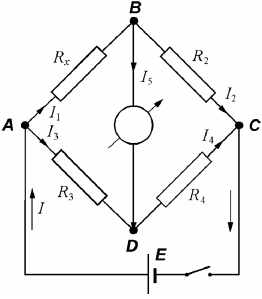
\includegraphics[scale=0.5]{mostek.png}}
\caption{Schemat oporowego mostka Wheatstone'a}
\label{fig:mostek}
\end{figure}

\section{Układ pomiarowy}

Na rysunku \ref{fig:uklad} przedstawiony jest przyrząd pomiarowy, w którym zastosowano drut oporowy wraz z linijką o dokładności $1 \unit{mm}$ służącą określeniu położenia punktu D od początku drutu (długość $a$). Długość drutu wynosi $l = 100 \unit{cm}$. Napięcie zasilania układu wynosiło $0,288 \unit{V}$. Opór $R_2$ stanowi opornica dekadowa. Symbolem $R_x$ oznaczono zestaw badanych oporników.

Jako, że w układzie zastosowano jednorodny drut oporowy równanie wartości poszukiwanego oporu możemy przedstawić jako:

$$ R_x = R_2\frac{a}{b} $$

Wiedząc, że $a + b = l$, możemy zapisać je w postaci:

$$ R_x = R_2\frac{a}{l - a} $$

\begin{figure}[!htp]
\centerline{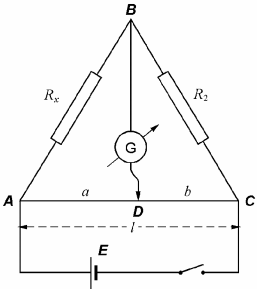
\includegraphics[scale=0.5]{uklad.png}}
\caption{Przyrząd pomiarowy - mostek Wheatstone'a z drutem oporowym}
\label{fig:uklad}
\end{figure}

\section{Wykonanie ćwiczenia}

\begin{enumerate}
  \item Podłączenie układu pomiarowego zgodnie ze schematem.
  \item Wykonanie dziesięciu pomiarów oporów dla różnych wartości $R_2$ dla każdego z badanych oporów.
\end{enumerate}

\section{Wyniki pomiarów}


\section{Wykresy}

\section{Opracowanie wyników}

\subsection{Analiza błędów}

Podczas analizy wyników nie znaleźliśmy błędów grubych. Natomiast analizując wykresy (rysunek ) możemy zauważyć, że zależność odległości $a$ od oporu wzorcowego w powtarzalny sposób odbiega od spodziewanej prostej. Wnioskujemy, że może być to związane z niejednorodnością zastosowanego drutu oporowego, bądź korozją wpływającą na opór punktu styku drutu z suwakiem.

\begin{figure}[!htp]
\centerline{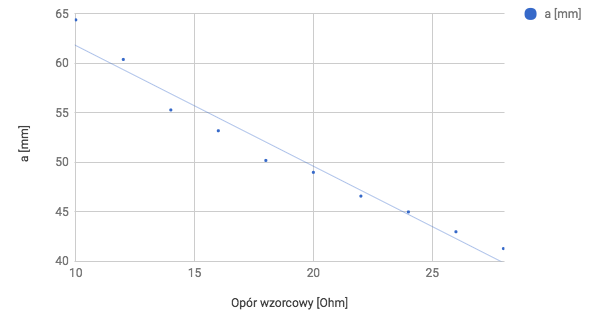
\includegraphics[scale=0.5]{wykres_r2.png}}
\caption{Zależność długości $a$ od oporu wzorcowego $R_2$}
\label{fig:wykres_r2}
\end{figure}

\begin{figure}[!htp]
\centerline{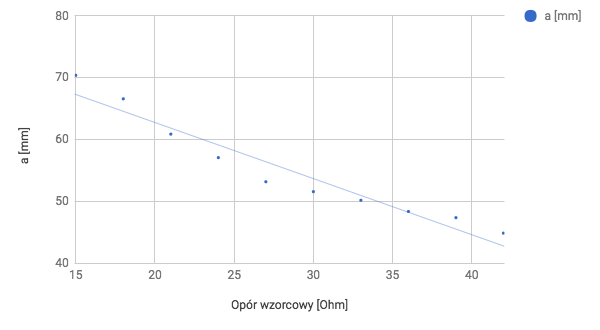
\includegraphics[scale=0.5]{wykres_r3.png}}
\caption{Zależność długości $a$ od oporu wzorcowego $R_3$}
\label{fig:wykres_r3}
\end{figure}

\begin{figure}[!htp]
\centerline{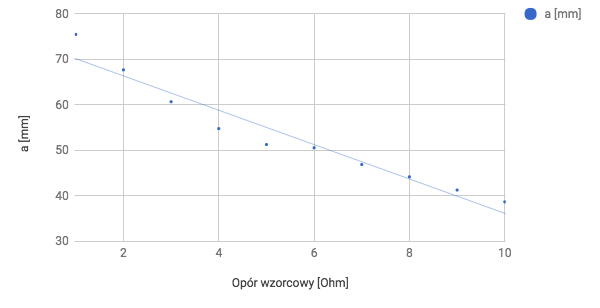
\includegraphics[scale=0.5]{wykres_r1_r2_par.png}}
\caption{Zależność długości $a$ od oporu wzorcowego $R_1, R_2$ połączonych równolegle}
\label{fig:wykres_r1_r2_par}
\end{figure}


\subsection{Niepewności pomiarów}

\subsection{Ocena zgodności uzyskanych wyników}

\section{Wnioski}

\end{document}
